%====================================================================================
\section[Modelo]{Un modelo de selección adversa}
%====================================================================================
\begin{frame}{Un modelo de selección adversa}
	Descripción del modelo
		\begin{center}
			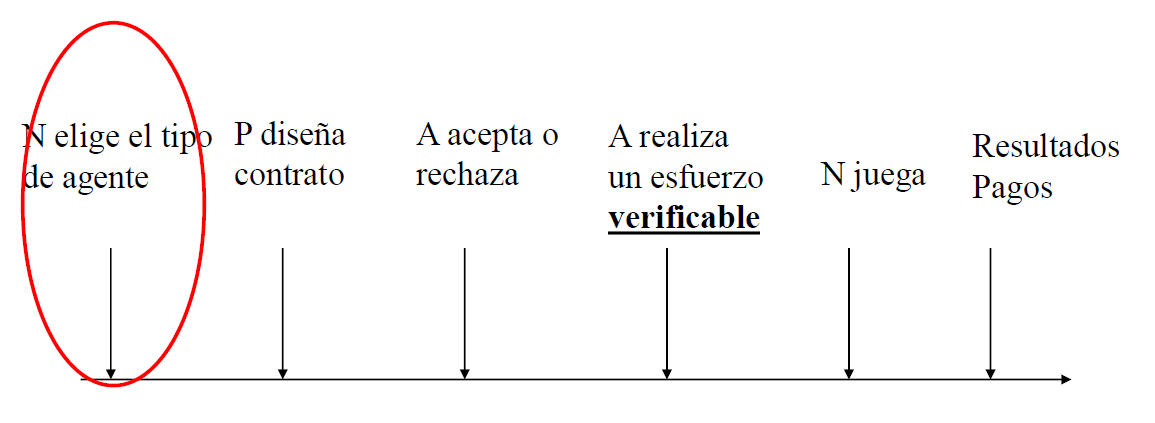
\includegraphics[width = 1\linewidth]{figures/fig_12.png}
		\end{center}
\end{frame}
%------------------------------------------------
\begin{frame}{Un modelo de selección adversa}
	Supuestos del modelo:
		\begin{enumerate}
			\item $P$ neutral al riesgo y $A$ es neutral o adverso.
			\item $P$ contrata al $A$ para que realice un esfuerzo verificable $(``e'')$.
			\item El $``e''$ genera un pago para $P$, de manera que el Beneficio bruto de P$ $cumple
					\begin{gather*}
						\frac{\pi(e)}{\pi^{\prime}(e)} > 0\\
						\pi^{\prime\prime}(e) \leq 0
					\end{gather*}
			\item El agente puede ser de dos tipos : bueno o malo.
			\item El principal desconoce de qué tipo es el agente.
		\end{enumerate}
\end{frame}
%------------------------------------------------
\begin{frame}{Un modelo de selección adversa}
	Agente bueno (con probabilidad $=q, 0<q<1$
		$$u^B(w,e) = u(w) - v(e)$$
	Agente malo (con probabilidad $= 1 -q$)
		$$u^M(w,e)=u(w)-kv(e) \quad , \quad k > 1$$
	Siendo
		\begin{itemize}
			\item u(w) = utilidad con respecto al salario.
			\item v(e) = desutilidad del esfuerzo
			\item k.v(e) > v(e)
		\end{itemize}
	Si el principal se enfrenta a un AGENTE BUENO resolverá el siguiente problema:
		\begin{align*}
			& \text{Max } \quad  \pi(e) - w\\
			& \begin{array}{ll}
				\text{s.a: } & u(w) - v(e) \geq \underline{U}
			\end{array}
		\end{align*}
\end{frame}
%------------------------------------------------
\begin{frame}{Un modelo de selección adversa}
	El Lagrangiano:
		$$\mathscr{L} = \pi(e) - w + \lambda\left[u(w) - v(e) - \underline{U} \right] $$
	CPO
		\begin{align}
			\frac{\partial \mathscr{L}}{\partial e}= 0 \rightarrow \pi^{\prime}(e) - \lambda v^{\prime}(e) = 0 \rightarrow \lambda = \frac{\pi^{\prime}(e)}{v^{\prime}(e)} \label{eq1}\\
			\frac{\partial \mathscr{L}}{\partial w}= 0 \rightarrow -1+\lambda u^{\prime}(w) = 0 \rightarrow \lambda = \frac{1}{u^{\prime}(e)} \label{eq2}
		\end{align}
	igualando (\ref{eq1}) y (\ref{eq2})
		$$\pi^{\prime}(e) = \frac{v^{\prime}(e)}{u^{\prime}(w)}$$
\end{frame}
%------------------------------------------------
\begin{frame}{Un modelo de selección adversa}
	El contrato óptimo que $P$ ofrece al agente, si supiese que es de tipo $B$, se determina resolviendo:
		\begin{center}
			\begin{tabular}{ccc}
				R.P. &{}& Condición de eficiencia\\
				$u(w^{B^{*}}) - v^{\prime}(e^{B^{*}}) = \underline{U}$&{}& $\pi^{\prime}(e^{B^{*}}) =\frac{v^{\prime}(e^{B^{*}})}{u^{\prime}(e^{B^{*}})}$
			\end{tabular}
		\end{center}
\end{frame}
%------------------------------------------------
\begin{frame}{Un modelo de selección adversa}
	Si el principal se enfrenta a un trabajador TIPO MALO resolverá el siguiente problema:
		\begin{align*}
			& \text{Max } \quad  \pi(e) - w\\
			& \begin{array}{ll}
				\text{s.a: } & u(w) - kv(e) \geq \underline{U}
			\end{array}
		\end{align*}
	El Lagrangiano:
		$$\mathscr{L} = \pi(e) - w + \lambda\left[u(w) - kv(e) - \underline{U} \right] $$
	CPO
		\begin{align}
			\frac{\partial \mathscr{L}}{\partial e}= 0 \rightarrow \pi^{\prime}(e) - \lambda kv^{\prime}(e) = 0 \rightarrow \lambda = \frac{\pi^{\prime}(e)}{kv^{\prime}(e)} \label{eq3}\\
			\frac{\partial \mathscr{L}}{\partial w}= 0 \rightarrow -1+\lambda u^{\prime}(w) = 0 \rightarrow \lambda = \frac{1}{u^{\prime}(e)} \label{eq4}
		\end{align}
\end{frame}
%------------------------------------------------
\begin{frame}{Un modelo de selección adversa}
	igualando (\ref{eq3}) y (\ref{eq4})
		$$\pi^{\prime}(e) = \frac{kv^{\prime}(e)}{u^{\prime}(w)}$$
	Contrato óptimo $(w^{M^\ast},e^{M^\ast})$
		\begin{center}
			\begin{tabular}{ccc}
				R.P. &{}& Condición de eficiencia\\
				$u(w^{M^{*}}) - kv^{\prime}(e^{M^{*}}) = \underline{U}$&{}& $\pi^{\prime}(e^{M^{*}}) =\frac{kv^{\prime}(e^{M^{*}})}{u^{\prime}(e^{M^{*}})}$
			\end{tabular}
		\end{center}
\end{frame}
%------------------------------------------------
\begin{frame}{Comparación gráfica:}
	\begin{center}
		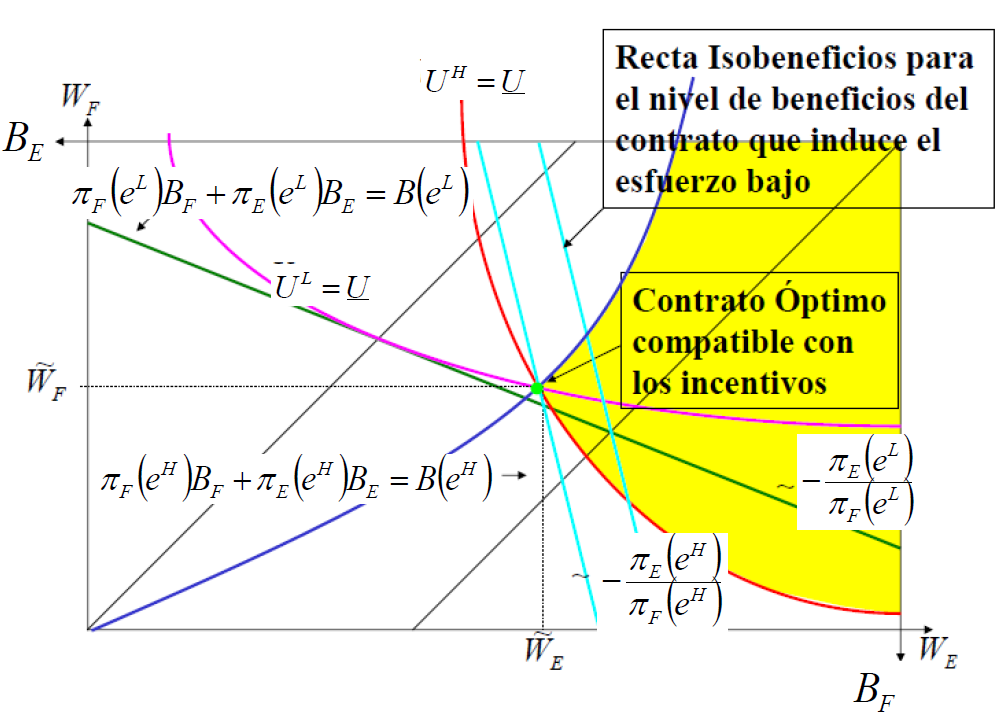
\includegraphics[width = 1\linewidth]{figures/fig_13.png}
	\end{center}
\end{frame}
%------------------------------------------------
\begin{frame}{Comparación gráfica:}
	Con información simétrica $P$ ofrecerá 2 contratos
	\begin{center}
		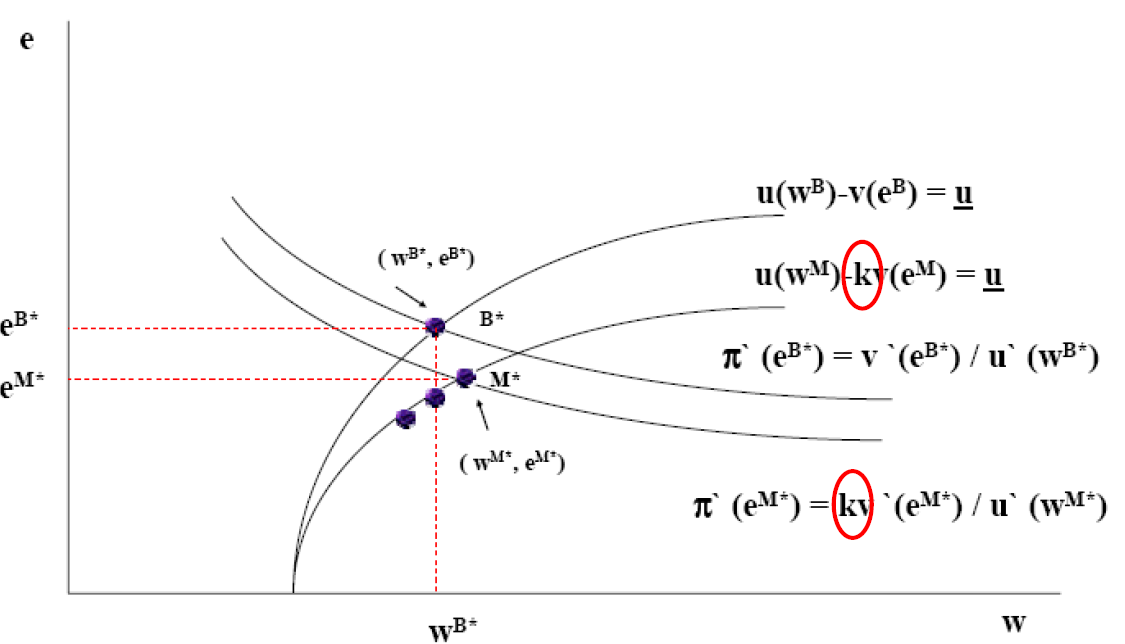
\includegraphics[width = 1\linewidth]{figures/fig_14.png}
	\end{center}
\end{frame}
%------------------------------------------------
\begin{frame}{Comparación gráfica:}
	Con información simétrica $P$ ofrecerá 2 contratos
	\begin{center}
		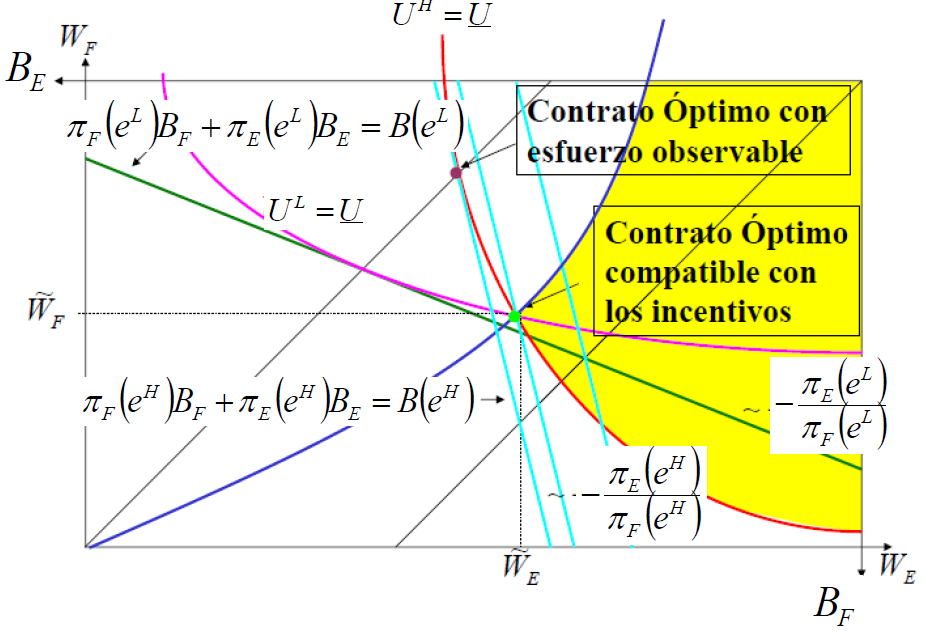
\includegraphics[width = 1\linewidth]{figures/fig_15.png}
	\end{center}
\end{frame}
%------------------------------------------------
\begin{frame}{Comparación gráfica:}
	Con información simétrica $P$ ofrecerá 2 contratos
	\begin{center}
		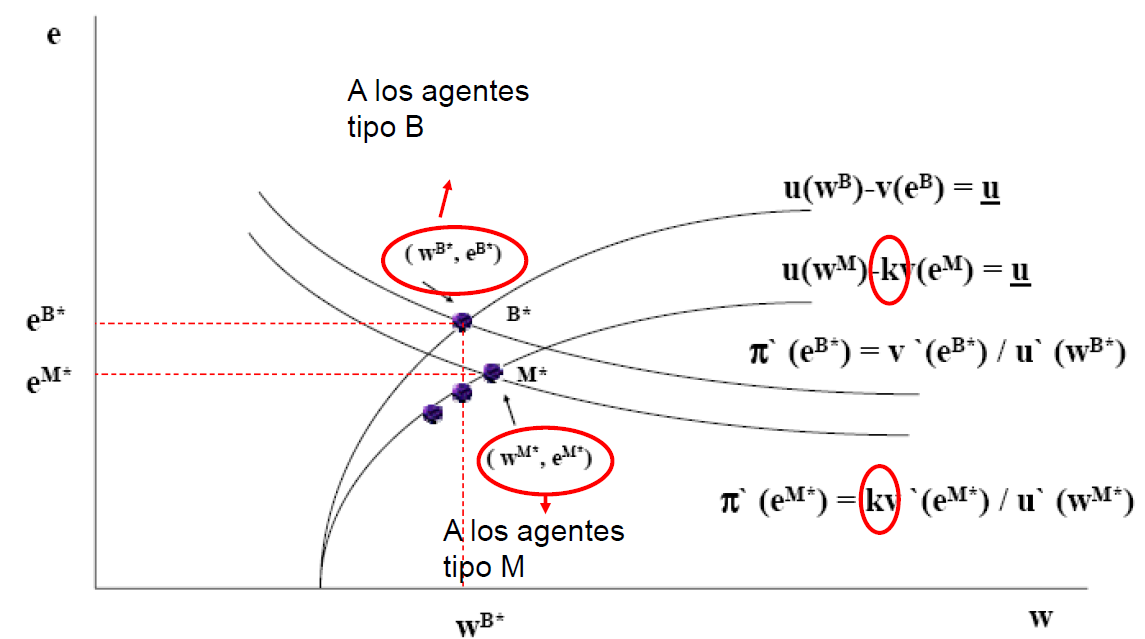
\includegraphics[width = 1\linewidth]{figures/fig_16.png}
	\end{center}
\end{frame}
%------------------------------------------------
\begin{frame}{Comparación gráfica:}
	\begin{center}
		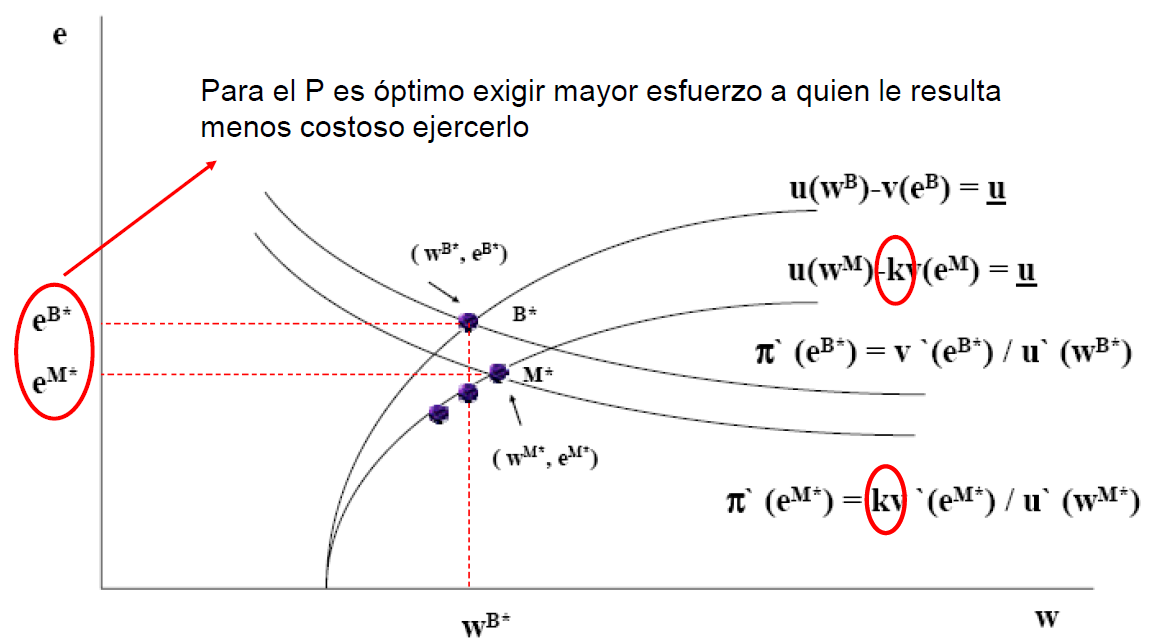
\includegraphics[width = 1\linewidth]{figures/fig_17.png}
	\end{center}
\end{frame}
%------------------------------------------------
\begin{frame}{Comparación gráfica:}
	\begin{center}
		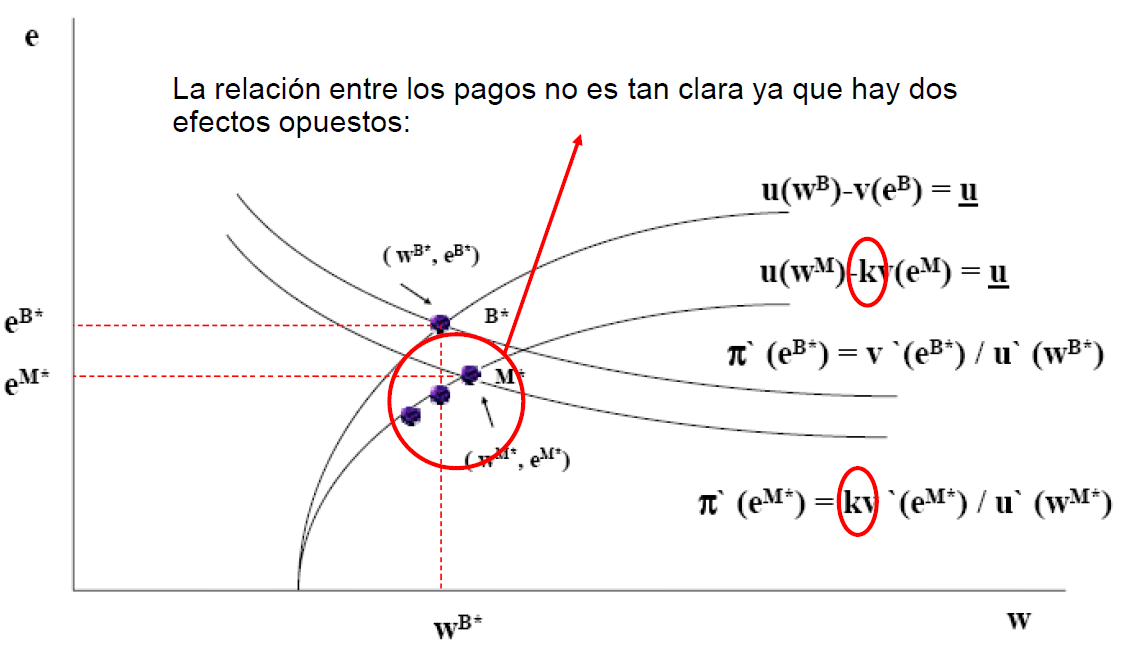
\includegraphics[width = 1\linewidth]{figures/fig_18.png}
	\end{center}
\end{frame}
%------------------------------------------------
\begin{frame}{Comparación gráfica:}
	\begin{center}
		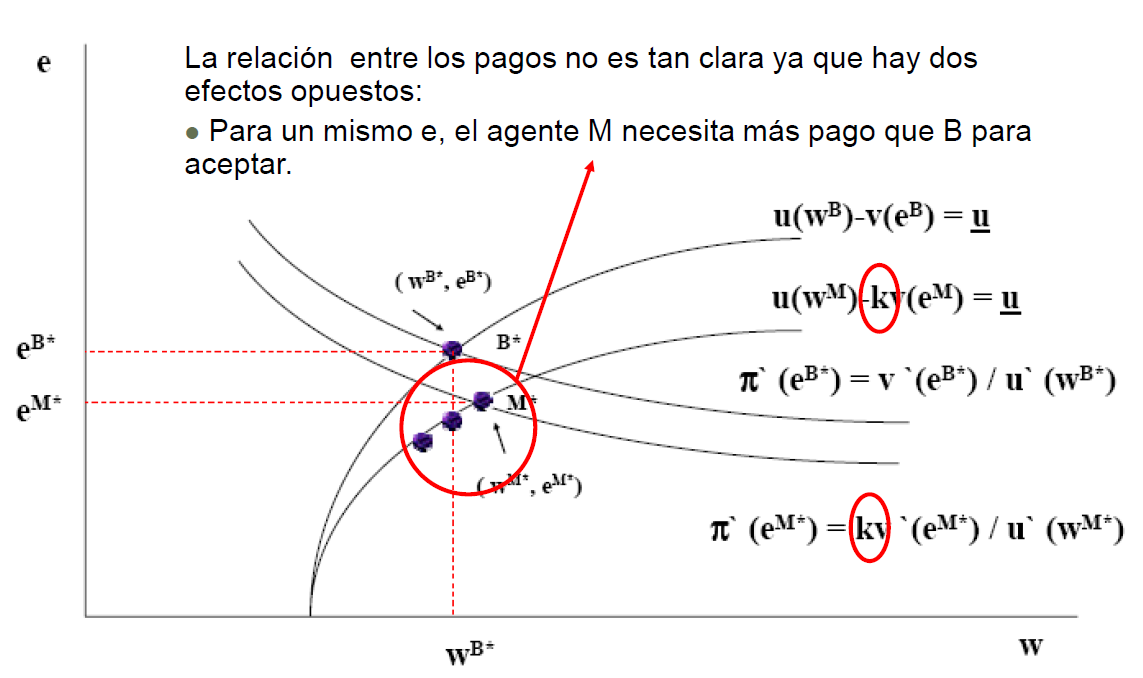
\includegraphics[width = 1\linewidth]{figures/fig_19.png}
	\end{center}
\end{frame}
%------------------------------------------------
\begin{frame}{Comparación gráfica:}
	\begin{center}
		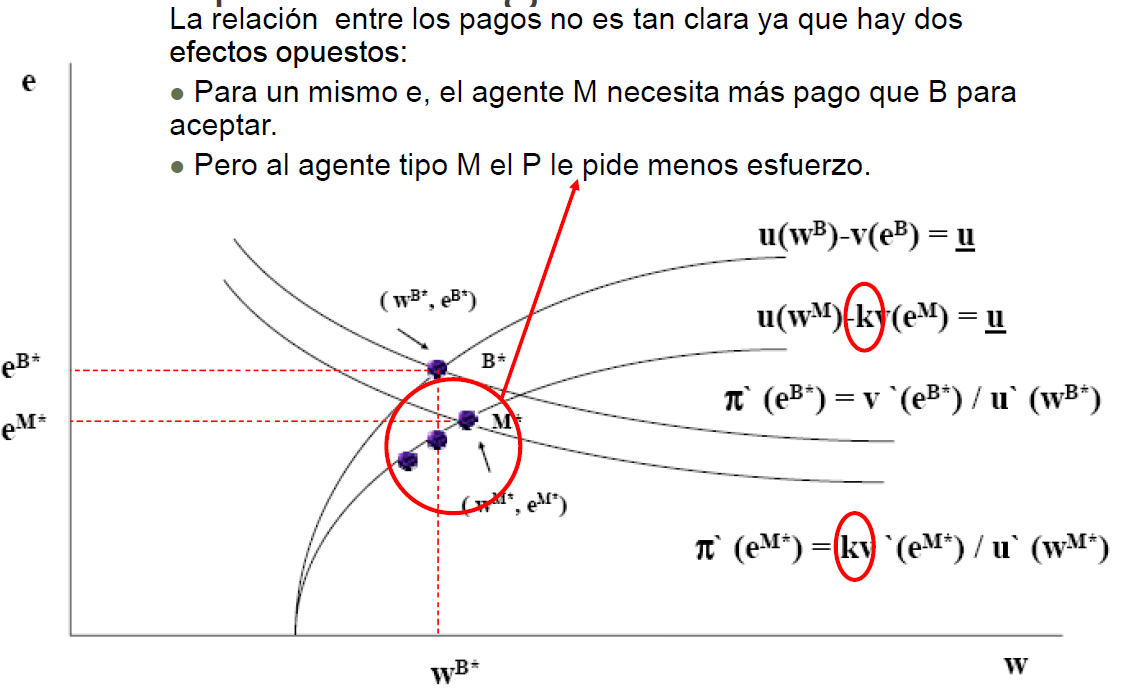
\includegraphics[width = 1\linewidth]{figures/fig_20.png}
	\end{center}
\end{frame}
%------------------------------------------------
\begin{frame}{Comparación gráfica:}
	\begin{center}
		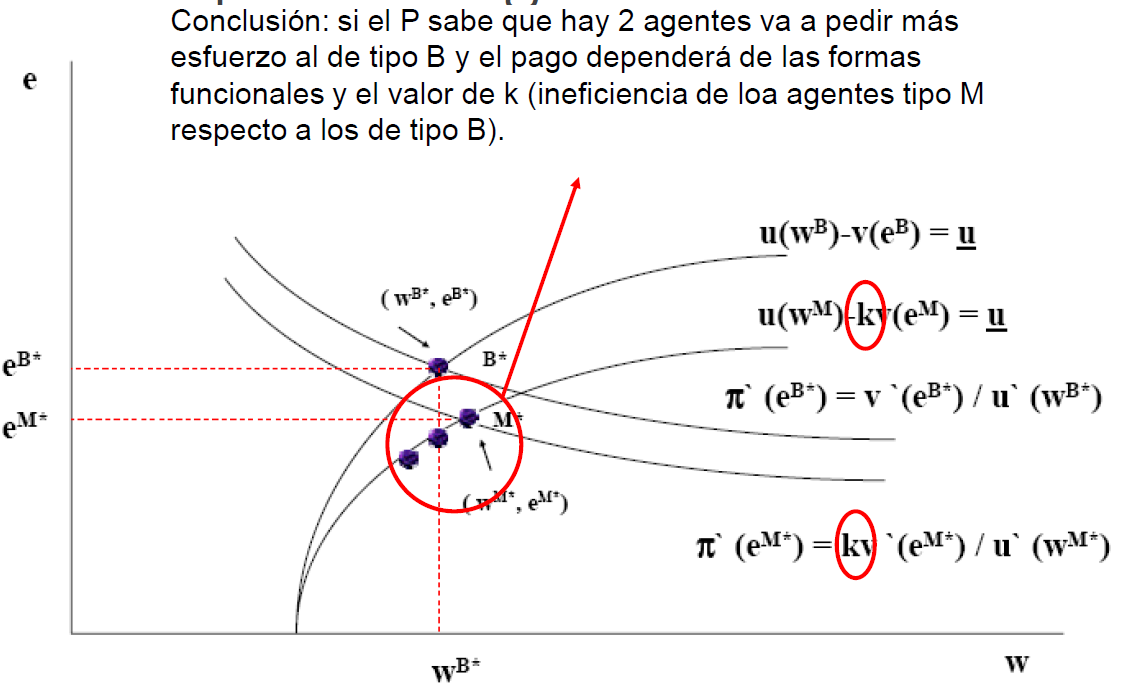
\includegraphics[width = 1\linewidth]{figures/fig_21.png}
	\end{center}
\end{frame}
%------------------------------------------------
\begin{frame}{Comparación gráfica:}
	Otra forma de verlo gráficamente:
	\begin{center}
		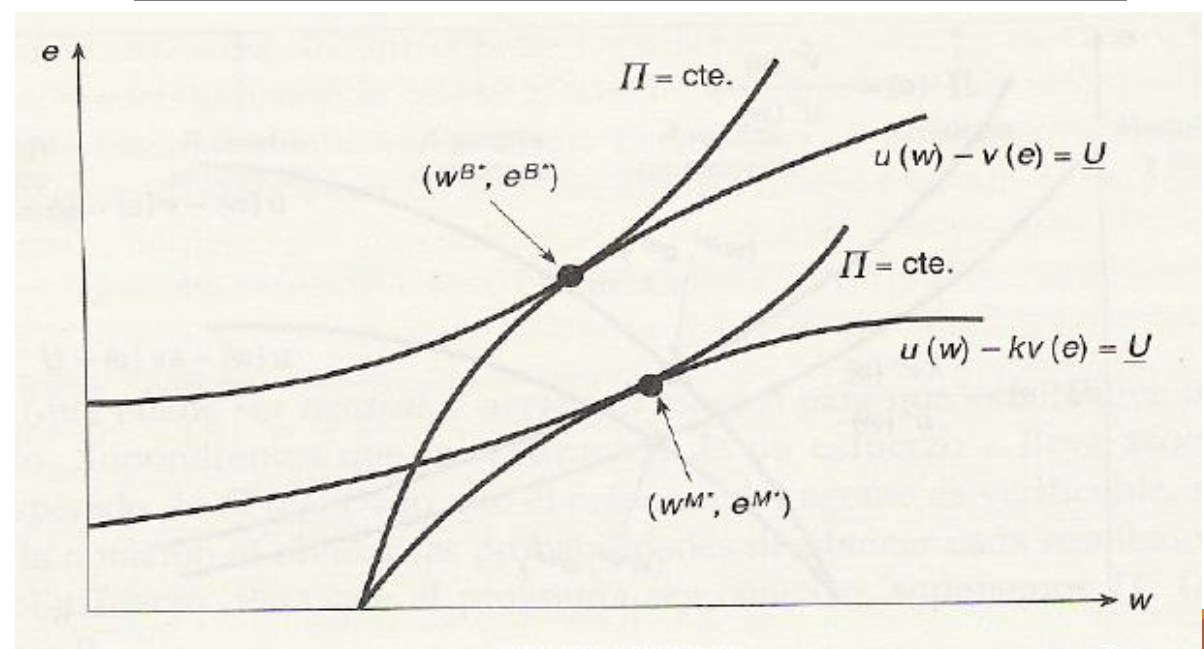
\includegraphics[width = 1\linewidth]{figures/fig_22.png}
	\end{center}
\end{frame}
%------------------------------------------------
\begin{frame}{Un modelo de selección adversa}
	Cuando hay asimetría de información si se ofrecen los contratos $B^*$ y $M^*$, tanto el agente $B$ como $M$ elegirán $(w^{M^\ast},e^{M^\ast})$ porque:
		$$U^B(w^{M^\ast},e^{M^\ast}) = u(w^{M^\ast}) - v(e^{M^\ast}) > u(w^{M^\ast}) - kv(e^{M^\ast}) = \underline{u}$$
	es decir:
		$$U^B(w^{M^\ast},e^{M^\ast}) > U^B(w^{B^\ast},e^{B^\ast}) = \underline{u}$$
\end{frame}
%------------------------------------------------
\begin{frame}{Un modelo de selección adversa}
	\begin{center}
		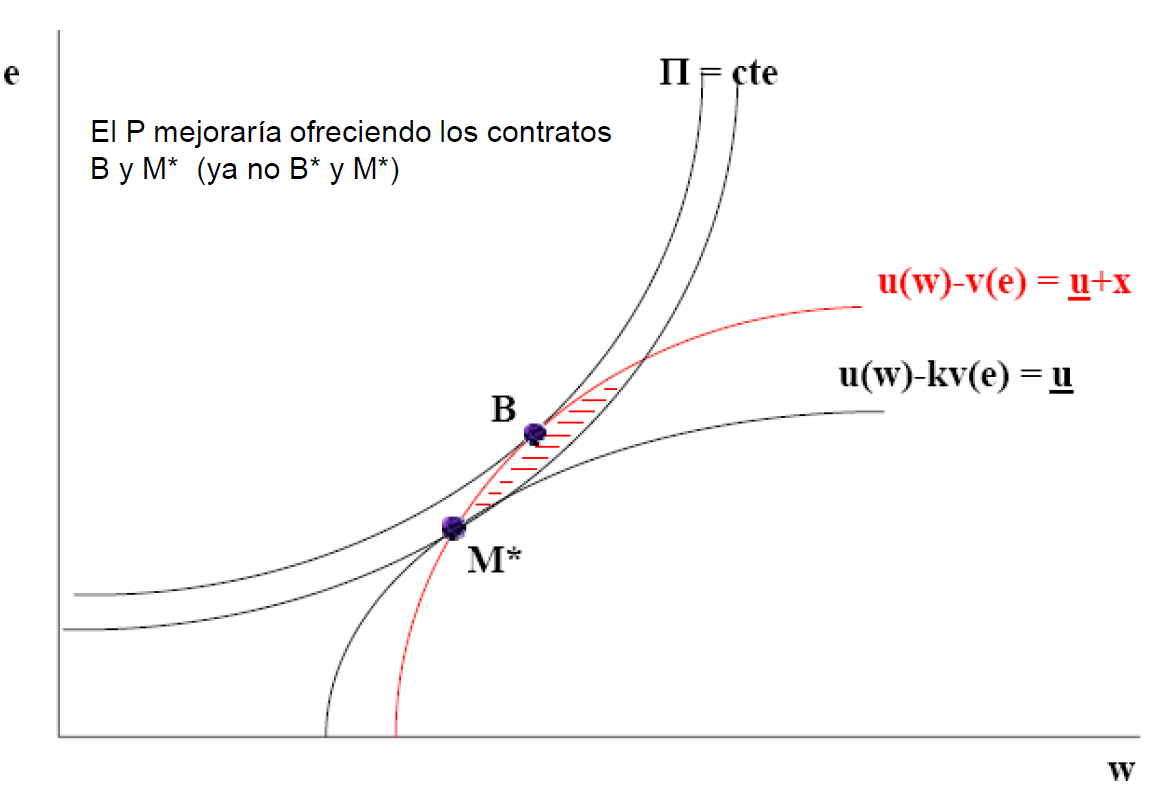
\includegraphics[width = 1\linewidth]{figures/fig_23.png}
	\end{center}
\end{frame}
%------------------------------------------------
\begin{frame}{Un modelo de selección adversa}
	Con información asimétrica lo mejor que puede hacer P es ofrecer un menú de contratos bien diseñados $(w^{M},e^{M})$ y $(w^{B},e^{B})$  tales que:
		\begin{itemize}
			\item $B$ elija $(w^{B},e^{B})$ prefiriéndolo a $(w^{M},e^{M})$
			\item $M$ elija $(w^{M},e^{M})$ prefiriéndolo a $(w^{M},e^{M})$
		\end{itemize}
	Se tratará de un esquema autoselectivo: cada agente al elegir mostrará sus verdaderas características.\\[0.3cm]
	El menú de contratos óptimo para el $P$ será un mecanismo revelador, pues consistirá en ofrecer contratos con los que consigue que cada agente revele sus verdaderas características.
\end{frame}
%------------------------------------------------
\begin{frame}{Un modelo de selección adversa}
	El diseño óptimo para el principal consiste en maximizar sus beneficios bajo las restricciones de que, tras ver los contratos, el agente decide entrar en relación con el principal y escoja aquel contrato que le va dirigido.
		$$\M \limits_{\left[(w^{M},e^{M}), (w^{B},e^{B}) \right]} q\left[ \Pi(e^B)-w^B\right] + (1-q)\left[ \Pi(e^M) - w^M\right] $$
	Siendo:
		\begin{itemize}
			\item $q=$ la proporción de individuos que eligen el contrato tipo bueno.
			\item $(1-q)$ = la proporción de individuos que eligen el contrato tipo malo
		\end{itemize}
\end{frame}
%------------------------------------------------
\begin{frame}{Un modelo de selección adversa}
	Sujeto a:
		\begin{itemize}
			\item las restricciones de aceptación que aseguran que los dos agentes acepten los contratos
			\item Las restricciones de incentivos, que aseguran que cada tipo de agente tenga interés en aceptar el contrato que le es dirigido
		\end{itemize}
	Entonces, las restricciones son
		\begin{gather}
			u(w^B) - v(e^B) \geq \underline{U} \label{eq5}\\
			u(w^M) - v(e^M) \geq \underline{U} \label{eq6}\\
			u(w^B) - v(e^B) \geq u(w^M) - v(e^M)\label{eq7}\\
			u(w^M) - v(e^M) \geq u(w^B) - v(e^B)\label{eq8}
		\end{gather}
\end{frame}
%------------------------------------------------
\begin{frame}{Un modelo de selección adversa}
	(\ref{eq5}) está implícita  en (\ref{eq6}) y (\ref{eq7})
		\begin{gather*}
			u(w^B) - v(e^B) \geq u(w^M) - v(e^M) > u(w^M) - v(e^M) \geq \underline{U}\\
			u(w^B) - v(e^B) \geq \underline{U}
		\end{gather*}
	Como esa restricción no se satura, no se tomará en cuenta en la resolución del problema.\\[0.3cm]
	Por tanto el lagrangiano será:
		\begin{align*}
			\mathscr{L} = & q\left[ \Pi(e^B)-w^B\right] + (1-q)\left[ \Pi(e^M) - w^M\right] +\\
						  & \lambda \left[u(w^M) - v(e^M) - \underline{U} \right] +\\
						  & \mu \left[ u(w^B) - v(e^B) - u(w^M) + v(e^M)\right] +\\
						  & \gamma \left[u(w^M) - v(e^M) - u(w^B) + v(e^B) \right] 
		\end{align*}
\end{frame}